\chapter{Scapegoat Trees}
\chaplabel{scapegoat}

In this chapter, we study a binary search tree data structure, the
#ScapegoatTree#.  This structure is based on the common wisdom that,
when something goes wrong, the first thing people tend to do is find
someone to blame (the \emph{scapegoat}).
\index{scapegoat}%
Once blame is firmly
established, we can leave the scapegoat to fix the problem.

A #ScapegoatTree# keeps itself balanced by \emph{partial rebuilding
operations}.
\index{partial rebuilding}%
\index{binary search tree!partial rebuilding}%
During a partial rebuilding operation, an entire subtree is
deconstructed and rebuilt into a perfectly balanced subtree.  There are
many ways of rebuilding a subtree rooted at node #u# into a perfectly
balanced tree.  One of the simplest is to traverse #u#'s subtree,
gathering all its nodes into an array, #a#, and then to recursively
build a balanced subtree using #a#.  If we let $#m#=#a.length#/2$,
then the element #a[m]# becomes the root of the new subtree,
$#a#[0],\ldots,#a#[#m#-1]$ get stored recursively in the left subtree
and $#a#[#m#+1],\ldots,#a#[#a.length#-1]$ get stored recursively in the
right subtree.
\codeimport{ods/ScapegoatTree.rebuild(u).packIntoArray(u,a,i).buildBalanced(a,i,ns)}
A call to #rebuild(u)# takes $O(#size(u)#)$ time.  The resulting subtree
has minimum height; there is no tree of smaller height that
has #size(u)# nodes.


\section{#ScapegoatTree#: A Binary Search Tree with Partial Rebuilding}
\seclabel{scapegoattree}


\index{ScapegoatTree@#ScapegoatTree#}%
A #ScapegoatTree# is a #BinarySearchTree# that, in addition to keeping
track of the number, #n#, of  nodes in the tree also keeps a counter, #q#,
that maintains an upper-bound on the number of nodes. 
\codeimport{ods/ScapegoatTree.q}
At all times, #n# and #q# obey the following inequalities:
\[
      #q#/2 \le  #n# \le #q#  \enspace .
\]
In addition, a #ScapegoatTree# has logarithmic height; at all times, the height of the scapegoat tree does not exceed
\begin{equation}
     \log_{3/2} #q# \le \log_{3/2} 2#n# < \log_{3/2} #n# + 2\enspace .
     \eqlabel{scapegoat-height}
\end{equation}
Even with this constraint, a #ScapegoatTree# can look surprisingly unbalanced.  The tree in \figref{scapegoat-example} has $#q#=#n#=10$ and height $5<\log_{3/2}10 \approx 5.679$.

\begin{figure}
  \begin{center}
    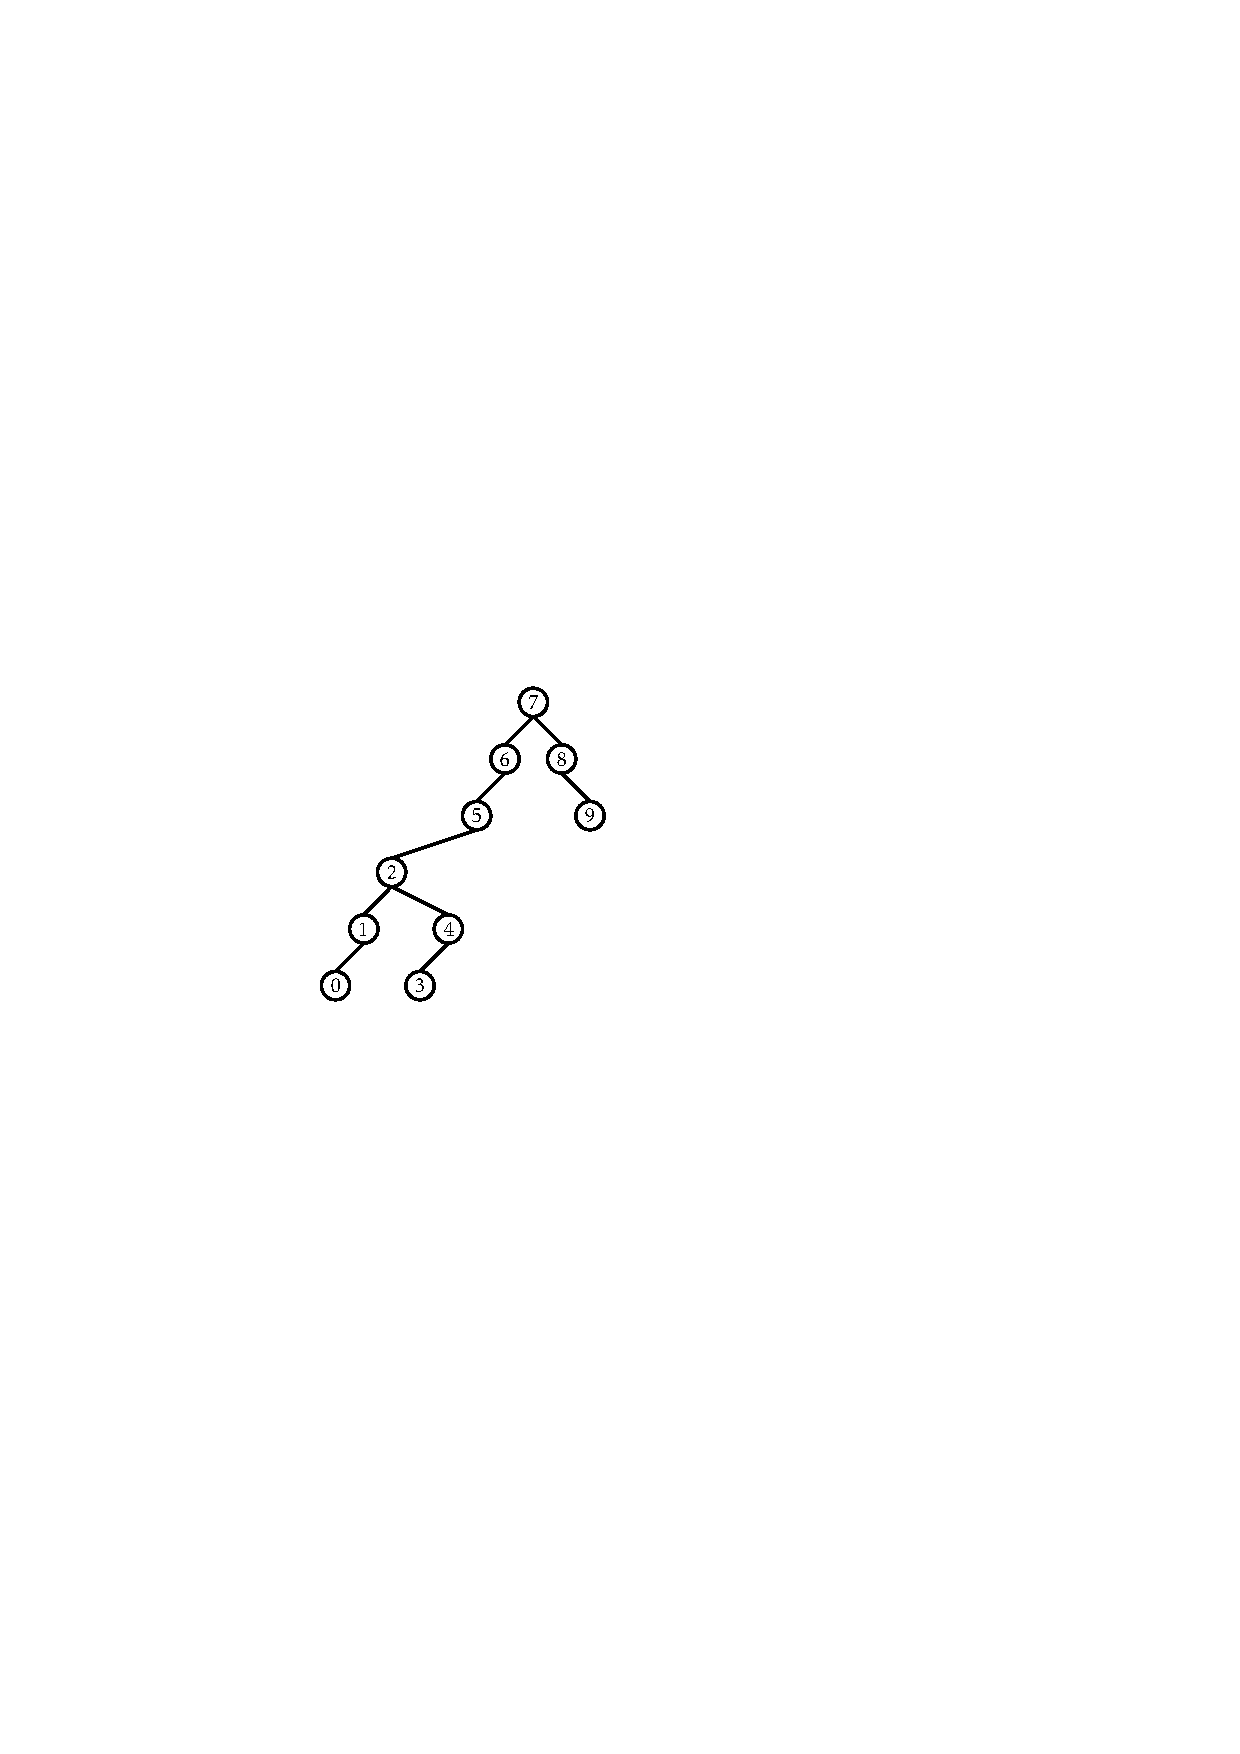
\includegraphics[scale=0.90909]{figs/scapegoat-insert-1}
  \end{center}
  \caption[A ScapegoatTree]{A #ScapegoatTree# with 10 nodes and height 5.}
  \figlabel{scapegoat-example}
\end{figure}

Implementing the #find(x)# operation in a #ScapegoatTree# is done
using the standard algorithm for searching in a #BinarySearchTree#
(see \secref{binarysearchtree}).  This takes time proportional to the
height of the tree which, by \myeqref{scapegoat-height} is $O(\log #n#)$.

To implement the #add(x)# operation, we first increment #n# and #q#
and then use the usual algorithm for adding #x# to a binary search
tree; we search for #x# and then add a new leaf #u# with $#u.x#=#x#$.
At this point, we may get lucky and the depth of #u# might not exceed
$\log_{3/2}#q#$. If so, then we leave well enough alone and don't do
anything else.

Unfortunately, it will sometimes happen that $#depth(u)# > \log_{3/2}
#q#$.  In this case, we need to reduce the height.  This isn't a big
job; there is only one node, namely #u#, whose depth exceeds $\log_{3/2}
#q#$.  To fix #u#, we walk from #u# back up to the root looking for a
\emph{scapegoat}, #w#.  The scapegoat, #w#, is a very unbalanced node.
It has the property that
\begin{equation}
   \frac{#size(w.child)#}{#size(w)#} > \frac{2}{3} \enspace ,
   \eqlabel{scapegoat}
\end{equation}
where #w.child# is the child of #w# on the path from the root to #u#.
We'll very shortly prove that a scapegoat exists.  For now, we can
take it for granted.  Once we've found the scapegoat #w#, we completely
destroy the subtree rooted at #w# and rebuild it into a perfectly balanced
binary search tree.  We know, from \myeqref{scapegoat}, that, even before
the addition of #u#, #w#'s subtree was not a complete binary tree.
Therefore, when we rebuild #w#, the height decreases by at least 1 so that the height of the #ScapegoatTree# is once again at most $\log_{3/2}#q#$.

\codeimport{ods/ScapegoatTree.add(x)}

\begin{figure}
  \begin{center}
    \begin{tabular}{cc}
      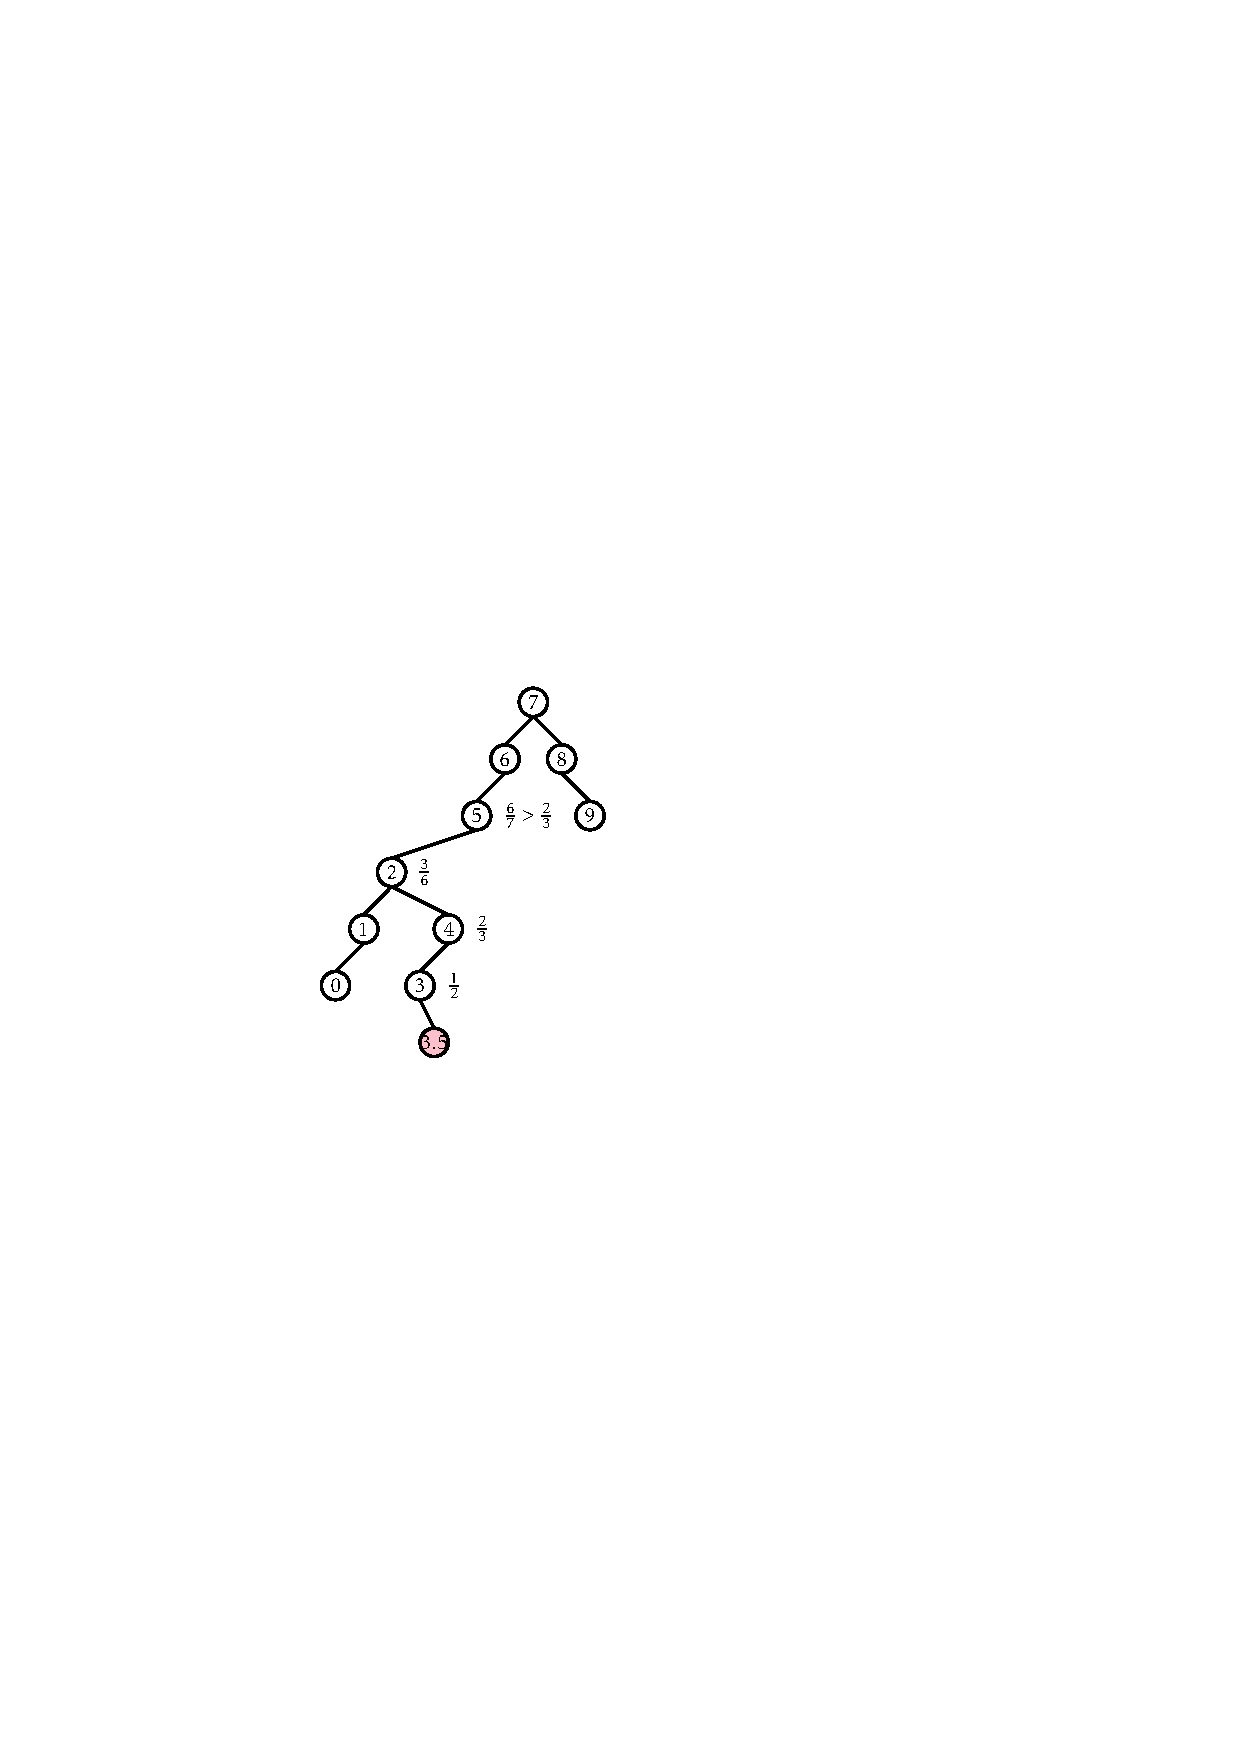
\includegraphics[scale=0.90909]{figs/scapegoat-insert-3} &
      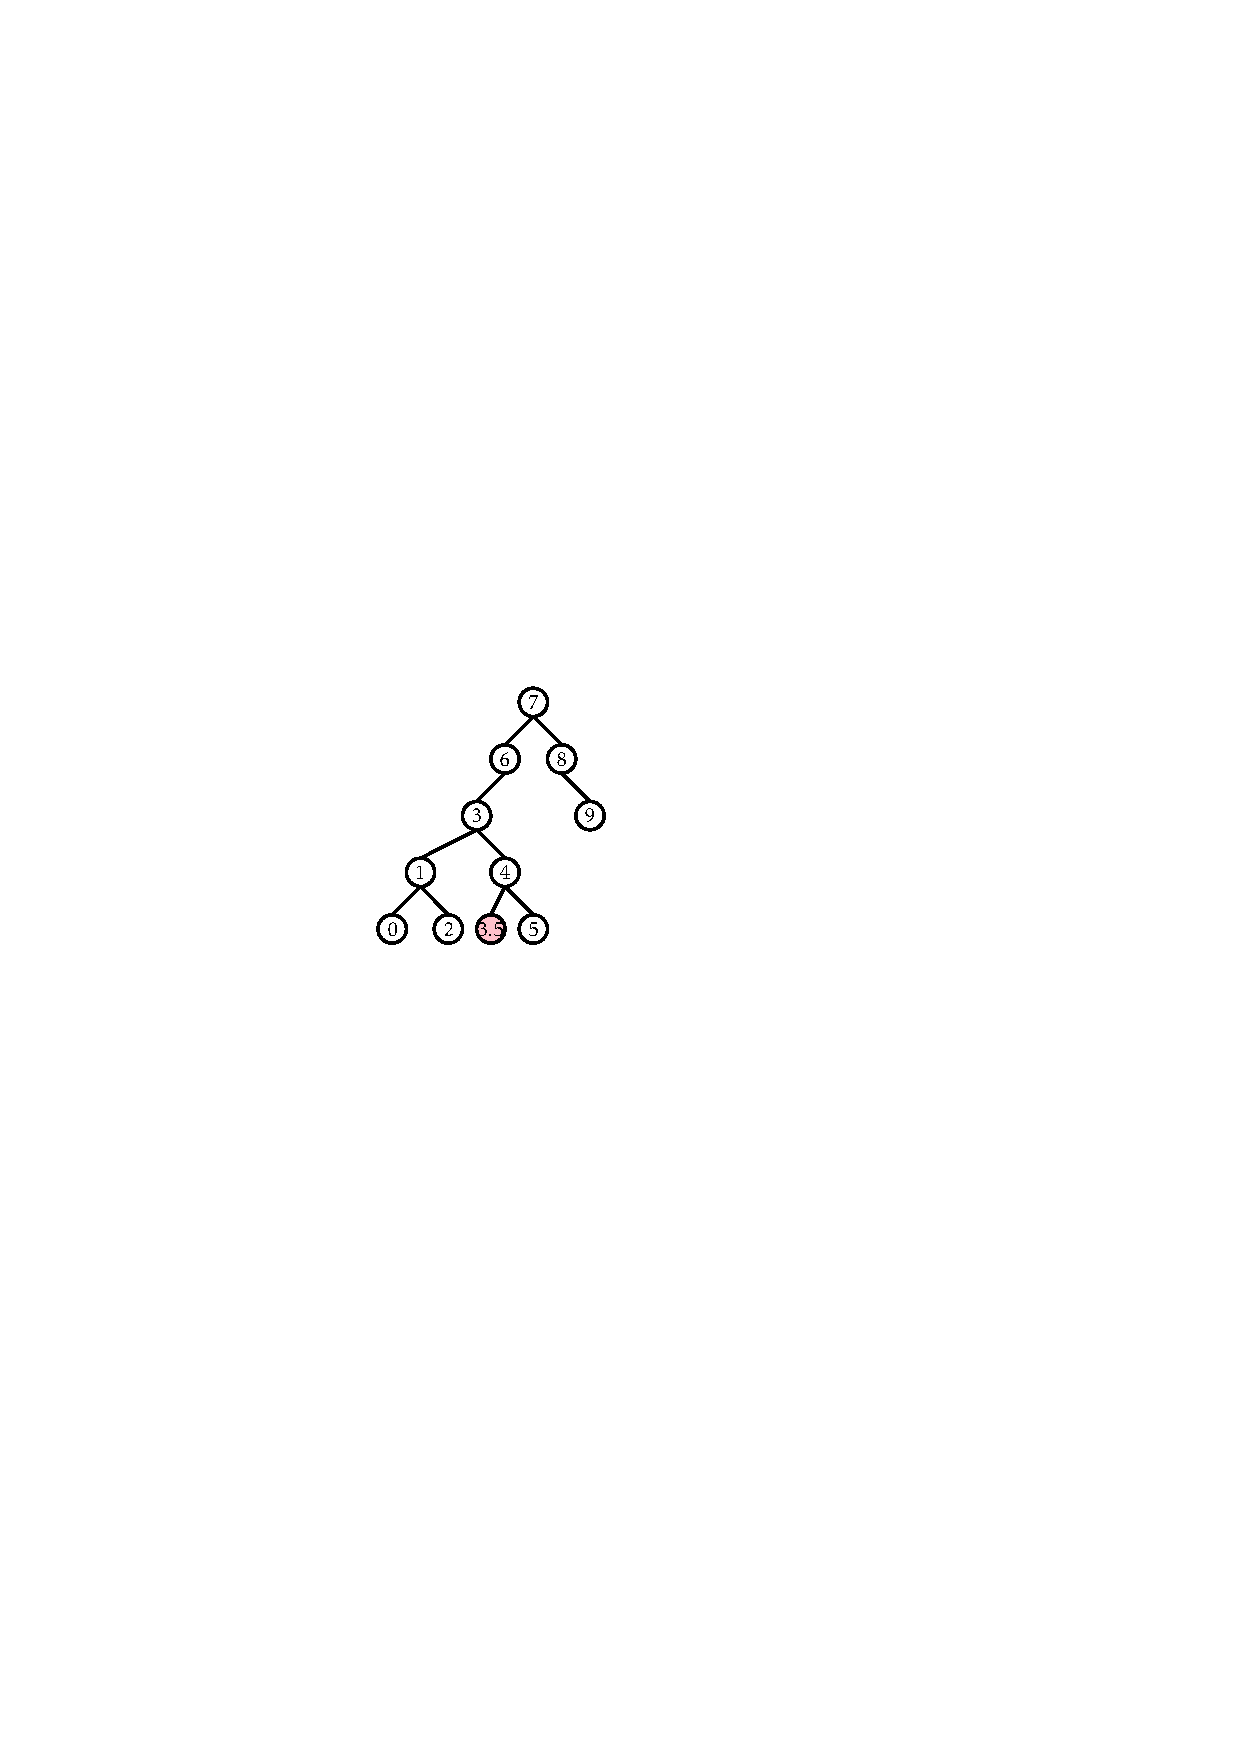
\includegraphics[scale=0.90909]{figs/scapegoat-insert-4} 
    \end{tabular}
  \end{center}
  \caption[Adding to a scapegoat tree]{Inserting 3.5 into a #ScapegoatTree# increases its height to 6, which violates \myeqref{scapegoat-height} since $6 > \log_{3/2} 11 \approx 5.914$.  A scapegoat is found at the node containing 5.}
\end{figure}
If we ignore the cost of finding the scapegoat #w# and rebuilding the
subtree rooted at #w#, then the running time of #add(x)# is dominated
by the initial search, which takes $O(\log #q#) = O(\log #n#)$ time.
We will account for the cost of finding the scapegoat and rebuilding
using amortized analysis in the next section.

The implementation of #remove(x)# in a #ScapegoatTree# is very simple.
We search for #x# and remove it using the usual algorithm for removing a
node from a #BinarySearchTree#.  (Note that this can never increase the
height of the tree.)  Next, we decrement #n#, but leave #q# unchanged.
Finally, we check if $#q# > 2#n#$ and, if so, then we \emph{rebuild the entire
tree} into a perfectly balanced binary search tree and set $#q#=#n#$.
\codeimport{ods/ScapegoatTree.remove(x)}
Again, if we ignore the cost of rebuilding, the running time of the
#remove(x)# operation is proportional to the height of the tree, and is
therefore $O(\log #n#)$.

\subsection{Analysis of Correctness and Running-Time}

In this section, we analyze the correctness and amortized running time
of operations on a #ScapegoatTree#.  We first prove the correctness by
showing that, when the #add(x)# operation results in a node that violates
Condition \myeqref{scapegoat-height}, then we can always find a scapegoat:

\begin{lem}
  Let #u# be a node of depth $h>\log_{3/2} #q#$ in a #ScapegoatTree#.
  Then there exists a node $#w#$ on the path from #u# to the root
  such that
  \[
     \frac{#size(w)#}{#size(parent(w))#} > 2/3 \enspace .
  \]
\end{lem}

\begin{proof}
  Suppose, for the sake of contradiction, that this is not the case, and
  \[
     \frac{#size(w)#}{#size(parent(w))#} \le 2/3 \enspace .
  \]
  for all nodes #w# on the path from #u# to the root.  Denote the path
  from the root to #u# as $#r#=#u#_0,\ldots,#u#_h=#u#$.  Then, we have
  $#size(u#_0#)#=#n#$,
  $#size(u#_1#)#\le\frac{2}{3}#n#$, 
  $#size(u#_2#)#\le\frac{4}{9}#n#$ and, more generally,
  \[
  #size(u#_i#)#\le\left(\frac{2}{3}\right)^i#n# \enspace .
  \]
  But this gives a contradiction, since $#size(u)#\ge 1$, hence
  \[
    1 \le #size(u)# \le \left(\frac{2}{3}\right)^h#n#
   < \left(\frac{2}{3}\right)^{\log_{3/2} #q#}#n#
   \le \left(\frac{2}{3}\right)^{\log_{3/2} #n#}#n#
   = \left(\frac{1}{#n#}\right) #n#
   = 1 \enspace . \qedhere
  \]
\end{proof}

Next, we analyze the parts of the running time that are not yet
accounted for.  There are two parts:  The cost of calls to #size(u)#
when searching for scapegoat nodes, and the cost of calls to #rebuild(w)#
when we find a scapegoat #w#.  The cost of calls to #size(u)# can be
related to the cost of calls to #rebuild(w)#, as follows:
\begin{lem}
During a call to #add(x)# in a #ScapegoatTree#, the cost of finding the scapegoat #w# and rebuilding the subtree rooted at #w# is $O(#size(w)#)$.
\end{lem}

\begin{proof}
The cost of rebuilding the scapegoat node #w#, once we find it, is
$O(#size(w)#)$.  When searching for the scapegoat node, we call #size(u)#
on a sequence of nodes $#u#_0,\ldots,#u#_k$ until we find the scapegoat
$#u#_k=#w#$.  However, since $#u#_k$ is the first node in this sequence
that is a scapegoat, we know that
\[
  #size(u#_{i}#)# < \frac{2}{3}#size(u#_{i+1}#)#
\]
for all $i\in\{0,\ldots,k-2\}$.  Therefore, the cost of all calls to #size(u)# is
\begin{eqnarray*}
 O\left( \sum_{i=0}^k #size(u#_{k-i}#)# \right)
 &=& O\left(
  #size(u#_k#)# 
  + \sum_{i=0}^{k-1} #size(u#_{k-i-1}#)#
  \right) \\
 &=& O\left(
  #size(u#_k#)# 
  + \sum_{i=0}^{k-1} \left(\frac{2}{3}\right)^i#size(u#_{k}#)#
  \right) \\
&=& O\left(
  #size(u#_k#)#\left(1+ 
   \sum_{i=0}^{k-1} \left(\frac{2}{3}\right)^i
  \right)\right) \\
&=& O(#size(u#_k#)#) = O(#size(w)#) \enspace ,
\end{eqnarray*}
where the last line follows from the fact that the sum is a geometrically decreasing series.
\end{proof}

All that remains is to prove an upper-bound on the cost of all calls to
#rebuild(u)# during a sequence of $m$ operations:

\begin{lem}\lemlabel{scapegoat-amortized}
  Starting with an empty #ScapegoatTree# any sequence of $m$ #add(x)#
  and #remove(x)# operations causes at most $O(m\log m)$ time to be used
  by #rebuild(u)# operations.
\end{lem}

\begin{proof}
  To prove this, we will use a \emph{credit scheme}.
  \index{credit scheme}%
  We imagine that each node
  stores a number of credits.  Each credit can pay for some constant,
  $c$, units of time spent rebuilding.  The scheme gives out a total of
  $O(m\log m)$ credits and every call to #rebuild(u)# is paid for with
  credits stored at #u#.

  During an insertion or deletion, we give one credit to each node on the
  path to the inserted node, or deleted node, #u#.  In this way we hand
  out at most $\log_{3/2}#q#\le \log_{3/2}m$ credits per operation.
  During a deletion we also store an additional credit ``on the side.''
  Thus, in total we give out at most $O(m\log m)$ credits.  All that
  remains is to show that these credits are sufficient to pay for all
  calls to #rebuild(u)#.

  If we call #rebuild(u)# during an insertion, it is because #u# is
  a scapegoat.  Suppose, without loss of generality, that
  \[
    \frac{#size(u.left)#}{#size(u)#} > \frac{2}{3} \enspace .
  \]
  Using the fact that
  \[
    #size(u)# = 1 + #size(u.left)# + #size(u.right)# 
  \]
  we deduce that
  \[
    \frac{1}{2}#size(u.left)# > #size(u.right)#  \enspace 
  \]
  and therefore
  \[
    #size(u.left)# - #size(u.right)# > \frac{1}{2}#size(u.left)# >
    \frac{1}{3}#size(u)#  \enspace .
  \]
  Now, the last time a subtree containing #u# was rebuilt (or when #u#
  was inserted, if a subtree containing #u# was never rebuilt), we had
  \[
    #size(u.left)# - #size(u.right)# \le 1 \enspace .
  \]
  Therefore, the number of #add(x)# or #remove(x)# operations that have
  affected #u.left# or #u.right# since then is at least
  \[
    \frac{1}{3}#size(u)# - 1 \enspace . 
  \]
  and there are therefore at least this many credits stored at #u#
  that are available to pay for the $O(#size(u)#)$ time it takes to
  call #rebuild(u)#.

  If we call #rebuild(u)# during a deletion, it is because $#q# > 2#n#$.
  In this case, we have $#q#-#n#> #n#$ credits stored ``on the side,'' and
  we use these to pay for the $O(#n#)$ time it takes to rebuild the root.
  This completes the proof.
\end{proof}

\subsection{Summary}
The following theorem summarizes the performance of the #ScapegoatTree# data structure:

\begin{thm}\thmlabel{scapegoat}
  A #ScapegoatTree# implements the #SSet# interface. Ignoring the cost
  of #rebuild(u)# operations, a #ScapegoatTree# supports the operations
  #add(x)#, #remove(x)#, and #find(x)# in $O(\log #n#)$ time per operation.
  
  Furthermore, beginning with an empty #ScapegoatTree#, any sequence of $m$
  #add(x)# and #remove(x)# operations results in a total of $O(m\log m)$
  time spent during all calls to #rebuild(u)#.
\end{thm}

\section{Discussion and Exercises}

The term \emph{scapegoat tree} is due to Galperin and Rivest \cite{gr93},
who define and analyze these trees.  However, the same structure
was discovered earlier by Andersson \cite{a89,a99}, who called them
\emph{general balanced trees}
\index{general balanced tree}%
since they can have any shape as long as
their height is small.

Experimenting with the #ScapegoatTree# implementation will reveal that
it is often considerably slower than the other #SSet# implementations
in this book. This may be somewhat surprising, since height bound of
\[
   \log_{3/2}#q# \approx 1.709\log #n# + O(1)
\] 
is better than the expected length of a search path in a #Skiplist# and
not too far from that of a #Treap#.  The implementation could be optimized
by storing the sizes of subtrees explicitly at each node or by reusing
already computed subtree sizes (Exercises~\ref{exc:scapegoat-quicksize}
and \ref{exc:scapegoat-explicitsize}).  Even with these optimizations,
there will always be sequences of #add(x)# and #delete(x)# operation for
which a #ScapegoatTree# takes longer than other #SSet# implementations.

This gap in performance is due to the fact that, unlike the other #SSet#
implementations discussed in this book, a #ScapegoatTree# can spend a lot
of time restructuring itself.  \excref{scapegoat-nlogn} asks you to prove
that there are sequences of #n# operations in which a #ScapegoatTree#
will spend on the order of $#n#\log #n#$ time in calls to #rebuild(u)#.
This is in contrast to other #SSet# implementations discussed in this
book, which only make $O(#n#)$ structural changes during a sequence
of #n# operations.  This is, unfortunately, a necessary consequence of
the fact that a #ScapegoatTree# does all its restructuring by calls to
#rebuild(u)# \cite{d90}.

Despite their lack of performance, there are applications in which a
#ScapegoatTree# could be the right choice.  This would occur any time
there is additional data associated with nodes that cannot be updated
in constant time when a rotation is performed, but that can be updated
during a #rebuild(u)# operation.  In such cases, the #ScapegoatTree#
and related structures based on partial rebuilding may work.  An example of such an application is outlined in \excref{list-order-maintenance}.

\begin{exc}
  Illustrate the addition of the values 1.5 and then 1.6 on the
  #ScapegoatTree# in \figref{scapegoat-example}.
\end{exc}

\begin{exc}
  Illustrate what happens when the sequence $1,5,2,4,3$ is added to an
  empty #ScapegoatTree#, and show where the credits described in the
  proof of \lemref{scapegoat-amortized} go, and how they are used during
  this sequence of additions.
\end{exc}

\begin{exc}\exclabel{scapegoat-nlogn}
  Show that, if we start with an empty #ScapegoatTree# and call #add(x)#
  for $#x#=1,2,3,\ldots,#n#$, then the total time spent during calls to
  #rebuild(u)# is at least $c#n#\log #n#$ for some constant $c>0$.
\end{exc}

\begin{exc}
  The #ScapegoatTree#, as described in this chapter, guarantees that the
  length of the search path does not exceed $\log_{3/2}#q#$.
  \begin{enumerate}
    \item  Design, analyze, and implement a modified version of
      #ScapegoatTree# where the length of the search path does not exceed
      $\log_{#b#} #q#$, where #b# is a parameter with $1<#b#<2$.
    \item What does your analysis and/or your experiments say about the
      amortized cost of #find(x)#, #add(x)# and #remove(x)# as a function
      of #n# and #b#?
  \end{enumerate}
\end{exc}

\begin{exc}\exclabel{scapegoat-quicksize}
  Modify the #add(x)# method of the #ScapegoatTree# so that it does not
  waste any time recomputing the sizes of subtrees that have already
  been computed.  This is possible because, by the time the method
  wants to compute #size(w)#, it has already computed one of #size(w.left)#
  or #size(w.right)#.  Compare the performance of your modified
  implementation with the implementation given here.
\end{exc}

\begin{exc}\exclabel{scapegoat-explicitsize}
  Implement a second version of the #ScapegoatTree# data structure that
  explicitly stores and maintains the sizes of the subtree rooted at
  each node.  Compare the performance of the resulting implementation
  with that of the original #ScapegoatTree# implementation as well as
  the implementation from \excref{scapegoat-quicksize}.
\end{exc}

\begin{exc}
  Reimplement the #rebuild(u)# method discussed at the beginning of this
  chapter so that it does not require the use of an array to store the
  nodes of the subtree being rebuilt.  Instead, it should use recursion
  to first connect the nodes into a linked list and then convert this
  linked list into a perfectly balanced binary tree.  (There are
  very elegant recursive implementations of both steps.)
\end{exc}

\begin{exc}
  \index{WeightBalancedTree@#WeightBalancedTree#}%
  Analyze and implement a #WeightBalancedTree#. This is a tree in
  which each node #u#, except the root, maintains the \emph{balance
  invariant} that $#size(u)# \le (2/3)#size(u.parent)#$.  The #add(x)# and
  #remove(x)# operations are identical to the standard #BinarySearchTree#
  operations, except that any time the balance invariant is violated at
  a node #u#, the subtree rooted at #u.parent# is rebuilt.
  Your analysis should show that operations on a #WeightBalancedTree#
  run in $O(\log#n#)$ amortized time.  
\end{exc}

\begin{exc}
  \index{CountdownTree@#CountdownTree#}%
  Analyze and implement a #CountdownTree#.  In a #CountdownTree# each
  node #u# keeps a \emph{timer} #u.t#.  The #add(x)# and #remove(x)#
  operations are exactly the same as in a standard #BinarySearchTree#
  except that, whenever one of these operations affects #u#'s subtree,
  #u.t# is decremented.  When $#u.t#=0$ the entire subtree rooted at #u#
  is rebuilt into a perfectly balanced binary search tree.  When a node
  #u# is involved in a rebuilding operation (either because #u# is rebuilt
  or one of #u#'s ancestors is rebuilt) #u.t# is reset to $#size(u)#/3$.

  Your analysis should show that operations on a #CountdownTree# run
  in $O(\log #n#)$ amortized time.  (Hint: First show that each node #u#
  satisfies some version of a balance invariant.)
\end{exc}

\begin{exc}
  \index{DynamiteTree@#DynamiteTree#}%
  Analyze and implement a #DynamiteTree#.  In a #DynamiteTree# each
  node #u# keeps tracks of the size of the subtree rooted at #u# in a
  variable #u.size#.  The #add(x)# and #remove(x)# operations are exactly
  the same as in a standard #BinarySearchTree# except that, whenever one
  of these operations affects a node #u#'s subtree, #u# \emph{explodes}
  with probability $1/#u.size#$.  When #u# explodes, its entire subtree
  is rebuilt into a perfectly balanced binary search tree.

  Your analysis should show that operations on a #DynamiteTree# run
  in $O(\log #n#)$ expected time. 
\end{exc}
 

\begin{exc}\exclabel{list-order-maintenance}
  \index{Sequence@#Sequence#}%
  Design and implement a #Sequence# data structure that maintains a
  sequence (list) of elements.  It supports these operations:
  \begin{itemize}
    \item #addAfter(e)#: Add a new element after the element #e# in the
    sequence.  Return the newly added element.  (If #e# is null,
    the new element is added at the beginning of the sequence.)
    \item #remove(e)#: Remove #e# from the sequence.
    \item #testBefore(e1,e2)#: return #true# if and only if #e1# comes
    before #e2# in the sequence.
  \end{itemize}
  The first two operations should run in $O(\log #n#)$ amortized time.
  The third operation should run in constant time.

  The #Sequence# data structure can be implemented by storing the elements
  in something like a #ScapegoatTree#, in the same order that they occur
  in the sequence.  To implement #testBefore(e1,e2)# in constant time,
  each element #e# is labelled with an integer that encodes the path from
  the root to #e#.  In this way, #testBefore(e1,e2)# can be implemented
  by comparing the labels of #e1# and #e2#.
\end{exc}

